\section{Introduction}\label{sec:intro}

A broad goal of machine learning research is to develop unified architectures capable of learning and reasoning over a wide range of tasks and data modalities, such as text, audio, time-series, and images. The generality of the input and output formats for sequence models such as Transformers~\citep{vaswani2017attention} makes them promising candidates for this goal. However, a tension exists between the goal of having a general architecture and the ability to support inductive biases that may be favorable for certain types of tasks. Recent research has shown that the standard Transformer architecture lacks the ability to efficiently learn and represent relational information, leading to several proposals for alternative architectures to encode inductive biases for relational learning \citep{santoroSimpleNeuralNetwork2017,santoroRelationalRecurrentNeural2018,shanahanExplicitlyRelationalNeurala,webbEmergentSymbolsBinding2021,webbRelationalBottleneckInductive2024,kergNeuralArchitectureInductive2022,altabaa2024abstractors,altabaaLearningHierarchicalRelational2024}. These relational architectures, on the other hand, fail to provide the generality required to handle more general learning tasks. In this paper, we present an extension of the Transformer architecture that preserves the generality of the architecture while integrating inductive biases for processing relational information between objects.

The Transformer can be understood as an instantiation of a broader computational paradigm implementing a neural message-passing algorithm that consists of iterative information retrieval followed by local processing. To process a sequence of objects $x_1,\ldots, x_n$, this takes the general form
\begin{equation}\label{eq:intro_message_passing}
  \begin{split}
    x_i &\gets \mathrm{Aggregate}\bigparen{x_i, \set{m_{j \to i}}_{j=1}^{n}} \\
    x_i &\gets \mathrm{Process}(x_i)
  \end{split}
\end{equation}
In the case of Transformers, the self-attention mechanism can be seen as sending messages from object $j$ to object $i$ that are encodings of the sender's features, with the message from sender $j$ to receiver $i$ given by $m_{j \to i} = \phi_v(x_j)$. These messages are then aggregated according to some selection criterion based on the receiver's features,  typically given by the softmax attention scores. In this work, we argue that there are two distinct types of information that need to be encoded in the messages $m_{j \to i}$. The first we refer to as \textit{sensory information}, which represents attributes or features of individual objects. The second is \textit{relational information} about the relationship between the sender and receiver along various dimensions.
% \footnote{This terminology of ``sensory'' and ``relational'' is borrowed from the cognitive neuroscience literature~\citep[e.g.,][]{holyoak2012analogy}. The generic term ``object'' is used to refer to elements of the input, which is typically a sequence or set. For example, objects might be the tokens in the context of text or the patches of an image in the context of vision.}. 
The Transformer architecture captures the transmission of sensory information, but does not explicitly support the transmission of relational information.

In this paper, we propose a novel type of attention mechanism that explicitly encodes learned relations between the sender and receiver. For this attention mechanism, the message from the sender object to the receiver object is a set of relations between them, which can be expressed as $m_{j \to i} = r(x_i, x_j)$, with the relations $r(\cdot,\cdot)$ computed through inner products of feature maps. By combining this with the standard attention mechanism of Transformers, we obtain a model that explicitly processes both sensory and relational information by stacking the two types of attention heads with $m_{j \to i} = (\phi_v(x_j), r(x_i, x_j))$. This \textit{Dual Attention} architecture disentangles the two types of information in the aggregation phase of attention, while making both types of information available during the information processing stage.

% \jlnote{More about Abstractors here, how we're building on it?}
% \aanote{maybe footnote directing reader to~\Cref{sec:appdx_abstrator}?}

% \aanote{note: for now, removed long paragraph summarizing experimental results}
% A series of four experiments across a range of data types demonstrates how the Dual Attention Transformer architecture preserves the benefits of standard Transformers while leading to greater efficiency of learning by combining relational information and sensory information. To begin, we use the Relational Games dataset which tests a model's ability to identify a particular visual relationship among a series of objects. We use a type of Vision Transformer architecture~\citep{dosovitskiyImageWorth16x162020}, and evaluate learning curves of the models, finding that the Dual Attention architecture is significantly more sample efficient compared to a standard Transformer. Next, we evaluate the Dual Attention architecture on a set of mathematical problem-solving tasks based on the benchmark contributed by~\citet{saxtonAnalyzingMathematicalReasoning2019}, where the tasks range \aanote*{typo}{from to} differentiating functions, finding that the Dual Attention models learn faster and reach higher accuracies compared to a standard Transformer. We also evaluate the new architecture on autoregressive language modeling. Using the Tiny Stories dataset of~\citet{eldanTinyStoriesHowSmall2023} to train models \aanote*{actually, our models are not on that scale, they're significantly smaller.}{on the roughly the scale of GPT-2}, we fix the total number of attention heads, and compare a Transformer with only standard self-attention heads to Dual Attention models with a mix of self-attention and relational attention heads, finding that the Dual Attention models achieve a smaller validation loss for the same total number of attention heads. Finally, we again use a Vision Transformer for classification of ImageNet images \citep{dosovitskiyImageWorth16x162020}, and find improved efficiency of learning. This suggests that relational processing is important in processing visual scenes, matching the intuition that parsing a visual scene requires reasoning about the visual relations between different objects or parts of the scene. Together, the experiments show that the Dual Attention Transformer is effective across a range of tasks and data types.

The contributions in this paper are summarized as follows:
\begin{enumerate}
  \item We introduce a new \textit{relational attention} mechanism that disentangles sensory information from relational information. While standard self-attention models retrieval of sensory information, relational attention models retrieval of relational information.
  \item We introduce a generalized Transformer architecture that integrates sensory and relational information through \textit{Dual Attention}---a form of multi-head attention with two distinct types of attention heads. Standard self-attention heads encode sensory information while relational attention heads encode relational information.
  \item We carry out an extensive set of experiments, showing that the \textit{Dual Attention Transformer} outperforms standard Transformers in terms of data efficiency. Our experiments range across several tasks and data modalities, including visual relational reasoning, symbolic mathematical reasoning, language modeling, and image recognition.
\end{enumerate}

% \aanote{note: for now, commented out paragraph about meaning of the terms ``sensory'', ``relational'', and ``objects''. TODO--find a place for it? e.g., footnote? or put back in intro?}
% Note that throughout the paper, the term ``sensory'' is used as shorthand to refer to the features and attributes of an individual object. For example, in a language task, this could be the components of a word embedding, and in a vision task, this could be the pixel values of a patch of an image or the feature maps obtained using a CNN. We use the term ``relational'' to refer to information about the relationship between the features of two objects. For example, in a language task, this could be the grammatical, syntactic, or semantic relation between two words. In a vision task, this could be a representation of similarity across different visual attributes such as the color, texture or semantic category of two objects. In the proposed learning architecture, the sensory information and relations are both learned, rather than being specified in advance of processing data for a given task.  The generic term ``object'' is used to refer to elements of the input, which is typically a sequence or set. For example, objects might be the tokens in the context of text or the patches of an image in the context of vision.

% \aawarning{TODO -- add sentence on potential congitive science connection? ``we borrow this language from recent work in the cognitive science literature, which argues that ...''}

% \aanote{\tiny{[An emerging idea in cognitive science] is that there essentially exists two distinct types of information when reasoning about collections of objects: ``sensory'' information concerning the attributes of individual objects, and ``relational'' information about the relationships between objects. It is contended that the first is associated with procedural knowledge whereas the second is associated abstraction. The standard attention mechanism of Transformers naturally captures retrieval of sensory information, but does not explicitly support reasoning about relational information.}}

\begin{figure}[t]
  \centering
  \begin{subfigure}[t]{0.415384615\textwidth} % 0.9 * 3 / 6.5
    \centering
    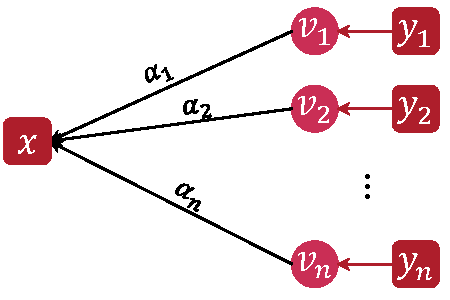
\includegraphics[width=\textwidth]{figs/sensory_retrieval.pdf} % size: 3 x 2 in
    \caption{$\Attn(x, \ys)$}%: Retrieval of sensory information by standard attention.}
  \end{subfigure}
  \qquad
  \begin{subfigure}[t]{0.484615385\textwidth} % 0.9 * 3.5 / 6.5
    \centering
    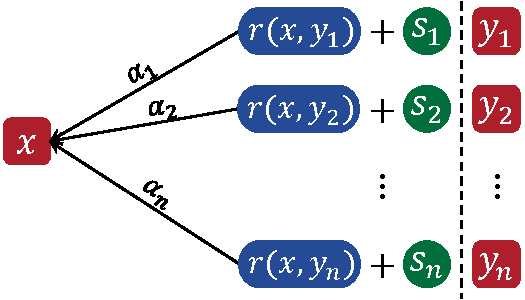
\includegraphics[width=\textwidth]{figs/relational_retrieval.pdf} % size 3.5 x 2 in
    \caption{$\RelAttn(x, \ys)$}%: Retrieval of relational information by relational attention.}
  \end{subfigure}
  % 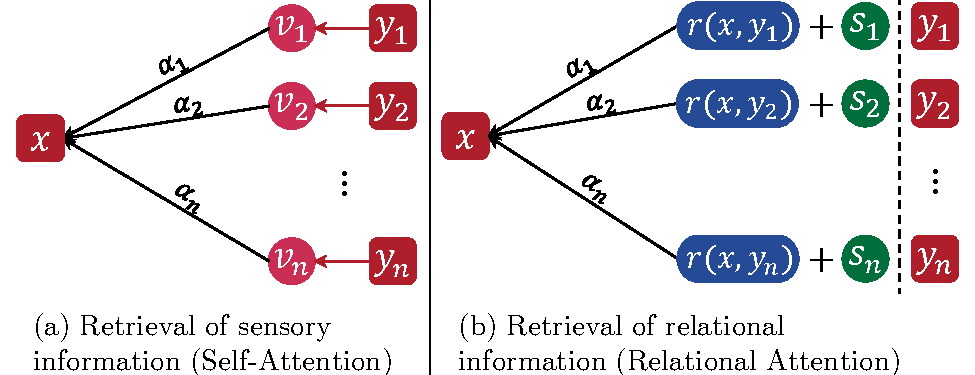
\includegraphics[width=0.8\textwidth]{figs/attn_fig_combined_noqeuerykey.pdf}
  \caption{Standard self-attention retrieves sensory information $v_i$ about the attributes of individual objects while \textit{relational attention} retrieves relational information $r(x, y_i)$ about the relationship between the objects in the context and the receiver.
  Each relation is tagged with a symbol $s_i$ which acts as an abstract variable identifying the sender.
  In both cases, information is aggregated according to the attention scores $\alpha_i$, which are computed by a softmax over inner products of queries and keys.
  }\label{fig:selfattn_relattn}
  \vskip-7pt
\end{figure}

% \aawarning{TODO---add footnote somewhere (maybe in section 2) referring reader to~\Cref{sec:appdx_abstrator} for a discussion on the relation to~\citet{altabaa2024abstractors}?}